\section{偏差与方差}
\label{sec:chapter9}

\subsection{训练集、验证集与测试集}

此前的实验使用全部数据训练模型，并在同一批数据上评估准确率。这种做法并不可靠：模型可能只是记住了训练样本，即使训练准确率很高，也可能已经发生过拟合，无法对新数据作出准确预测。正确的做法是保留一个不参与训练的独立测试集，只在模型建立完成后使用它进行最终评估，这样得到的结果才能反映模型的泛化能力。

如果模型包含需要人工选择的超参数，例如正则化参数 $\lambda$，仅划分训练集和测试集仍然不够。若反复根据测试结果选择表现最好的超参数，参数选择过程实际上也利用了测试集信息，测试集便不再真正独立。为此还要引入验证集：使用训练集拟合模型，使用验证集比较不同超参数，确定最终方案后再在测试集上评估。测试集自始至终都不参与模型训练和超参数选择。

如果训练过程包含正则项，计算训练集、验证集或测试集误差时应去除该项。正则化的作用是在训练阶段约束参数 $\theta$，帮助得到复杂度更合适的模型；而评价这个参数的实际预测效果时，真正需要衡量的是预测值与真实值之间的差异，因此应使用不含正则项的原始代价函数。

\subsection{高偏差与高方差}

模型发生欠拟合时，通常称其具有高偏差；发生过拟合时，则称其具有高方差。以多项式回归为例，随着多项式次数增加，模型表达能力逐渐增强，并由欠拟合过渡到合适拟合，最终可能出现过拟合。在这一过程中，训练误差 $J_\text{train}(\theta)$ 通常持续减小，因为更复杂的模型总能更充分地拟合训练数据；验证误差 $J_\text{valid}(\theta)$ 则会先减小后增大，在中间某个复杂度处达到最小值，如下图所示：

\begin{figure}[H]
    \centering
    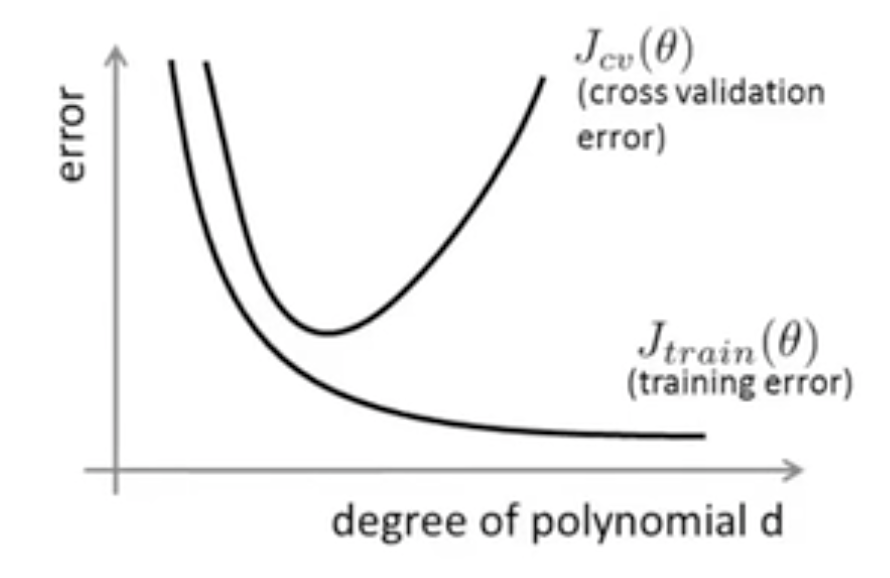
\includegraphics[width=0.4\linewidth]{figs/Chap_9_img.png}
\end{figure}

\subsection{学习曲线}

误差随训练集规模变化的曲线称为学习曲线。分别绘制训练误差与验证误差，可以观察增加训练数据时模型表现如何变化，从而帮助判断模型处于高偏差还是高方差状态。

对于高偏差模型，当训练集很小时，模型容易拟合少量样本，因此 $J_\text{train}(\theta)$ 较小，而 $J_\text{valid}(\theta)$ 较大。随着训练集增大，训练任务变得更困难，$J_\text{train}(\theta)$ 会迅速增大；$J_\text{valid}(\theta)$ 虽然有所减小，但幅度通常有限。最终二者逐渐接近，并共同稳定在较高水平，说明模型本身的表达能力不足。

对于高方差模型，训练集很小时，模型可以近乎记住所有样本，因此 $J_\text{train}(\theta)$ 很小，而 $J_\text{valid}(\theta)$ 较大。随着训练集增大，$J_\text{train}(\theta)$ 会略有上升，$J_\text{valid}(\theta)$ 会逐渐下降；但即使训练集已经较大，训练误差仍可能明显小于验证误差，二者之间保持较大间隔。

\begin{figure}[H]
    \centering
    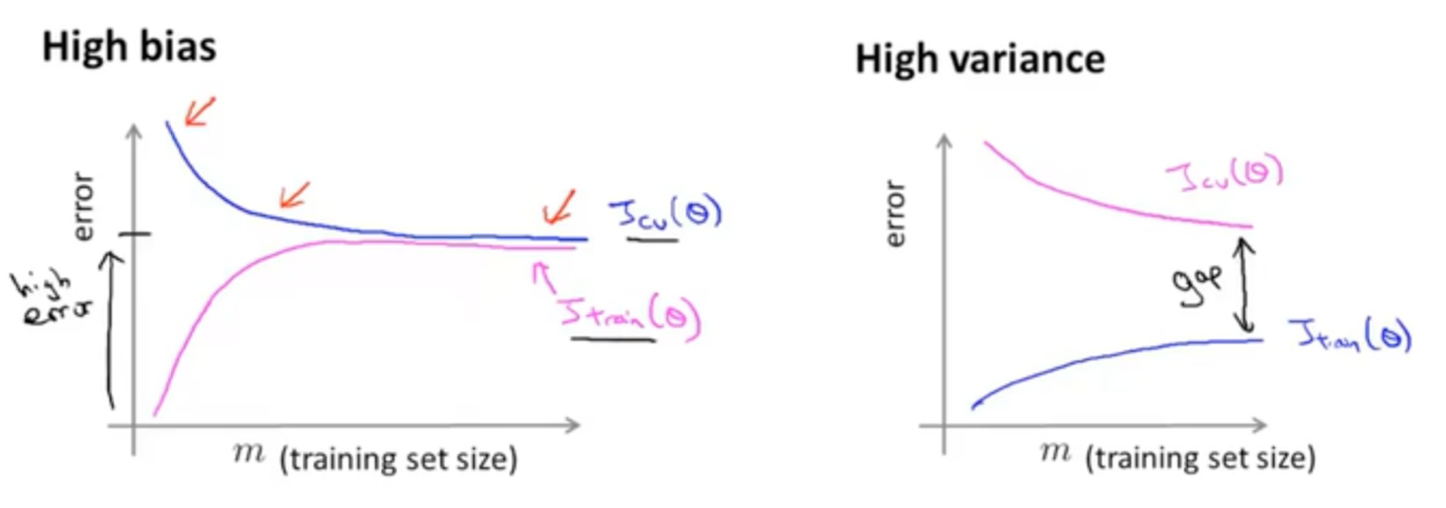
\includegraphics[width=0.8\linewidth]{figs/Chap_9_img2.png}
\end{figure}

由上述分析可知，如果模型处于高偏差状态，继续增加训练数据通常没有明显帮助，因为模型本身过于简单；更有效的方法是增加特征或提高模型复杂度。对于高方差模型，增加训练数据则可能缩小训练误差与验证误差之间的差距，从而缓解过拟合。


\subsection{代码实现}

\paragraph{正则化线性回归}

首先观察数据集：

\begin{figure}[H]
    \centering
    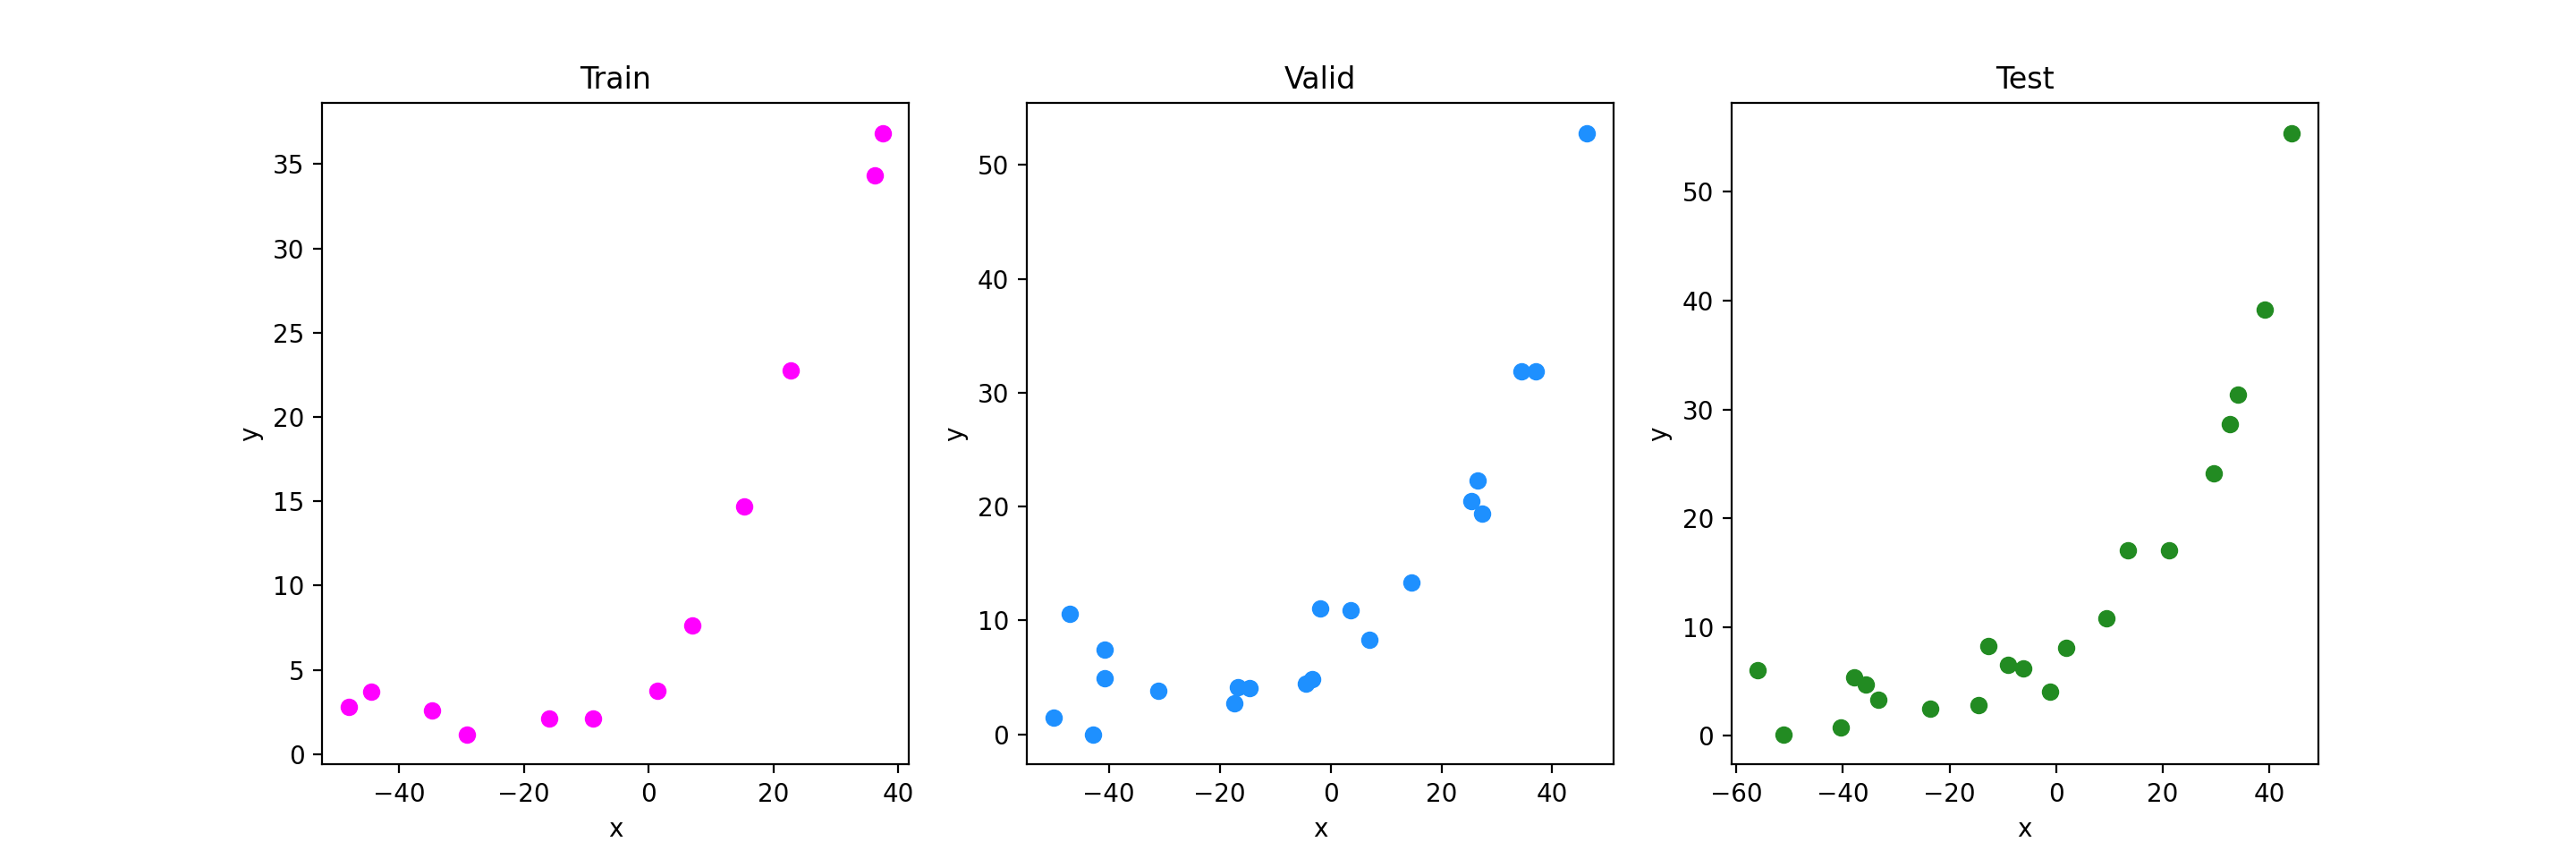
\includegraphics[width=\linewidth]{figs/Chap_9_Figure_0.png}
\end{figure}

正则化线性回归的矩阵形式为：
\begin{align*}
J(\theta)&=\frac{1}{2m}\left[\theta^TX^TX\theta-2\theta^TX^Ty+y^Ty+\lambda\hat\theta^T\hat\theta\right]\\
\frac{\partial J}{\partial \theta}&=\frac{1}{m}\left[X^TX\theta-X^Ty+\lambda\hat\theta\right]
\end{align*}

其中，$\hat\theta$ 表示将 $\theta_0$ 置为 $0$ 后的 $\theta$，因为偏置项不参与正则化。

\begin{lstlisting}[language=Python]
import numpy as np
from scipy.io import loadmat
from scipy.optimize import minimize
import matplotlib.pyplot as plt

data = loadmat('ex5data1.mat')
X, y, Xval, yval, Xtest, ytest = \
data['X'], data['y'], data['Xval'], data['yval'], data['Xtest'], data['ytest']
X = np.hstack((np.ones((X.shape[0], 1)), X))
Xval = np.hstack((np.ones((Xval.shape[0], 1)), Xval))
Xtest = np.hstack((np.ones((Xtest.shape[0], 1)), Xtest))

def unseq(theta):
	return theta.reshape(theta.shape[0], 1)

def seq(theta):
	return theta.flatten()

def J(theta, X, y, lamb):
	m = X.shape[0]
	thetahat = np.vstack((np.zeros((1, 1)), theta[1:, :]))
	return ((theta.T@X.T@X@theta-2*theta.T@X.T@y+y.T@y+lamb*thetahat.T@thetahat)/m/2)[0][0]

def partJ(theta, X, y, lamb):
	m = X.shape[0]
	thetahat = np.vstack((np.zeros((1, 1)), theta[1:, :]))
	return (X.T@X@theta-X.T@y+lamb*thetahat)/m

def Train(X, y):
	return minimize(fun = lambda theta, X, y, lamb: J(unseq(theta), X, y, lamb), 
				   x0 = np.array([1, 1]), 
				   jac = lambda theta, X, y, lamb: seq(partJ(unseq(theta), X, y, lamb)), 
				   args = (X, y, 1), 
				   method = 'CG')

res = Train(X, y)
print(res)
\end{lstlisting}

回归结果为：

\begin{lstlisting}
     fun: 22.3795418229475
     jac: array([ 3.74520898e-06, -1.25949765e-07])
 message: 'Optimization terminated successfully.'
    nfev: 28
     nit: 18
    njev: 28
  status: 0
 success: True
       x: array([13.08771802,  0.36774202])
\end{lstlisting}

回归曲线如下：

\begin{figure}[H]
    \centering
    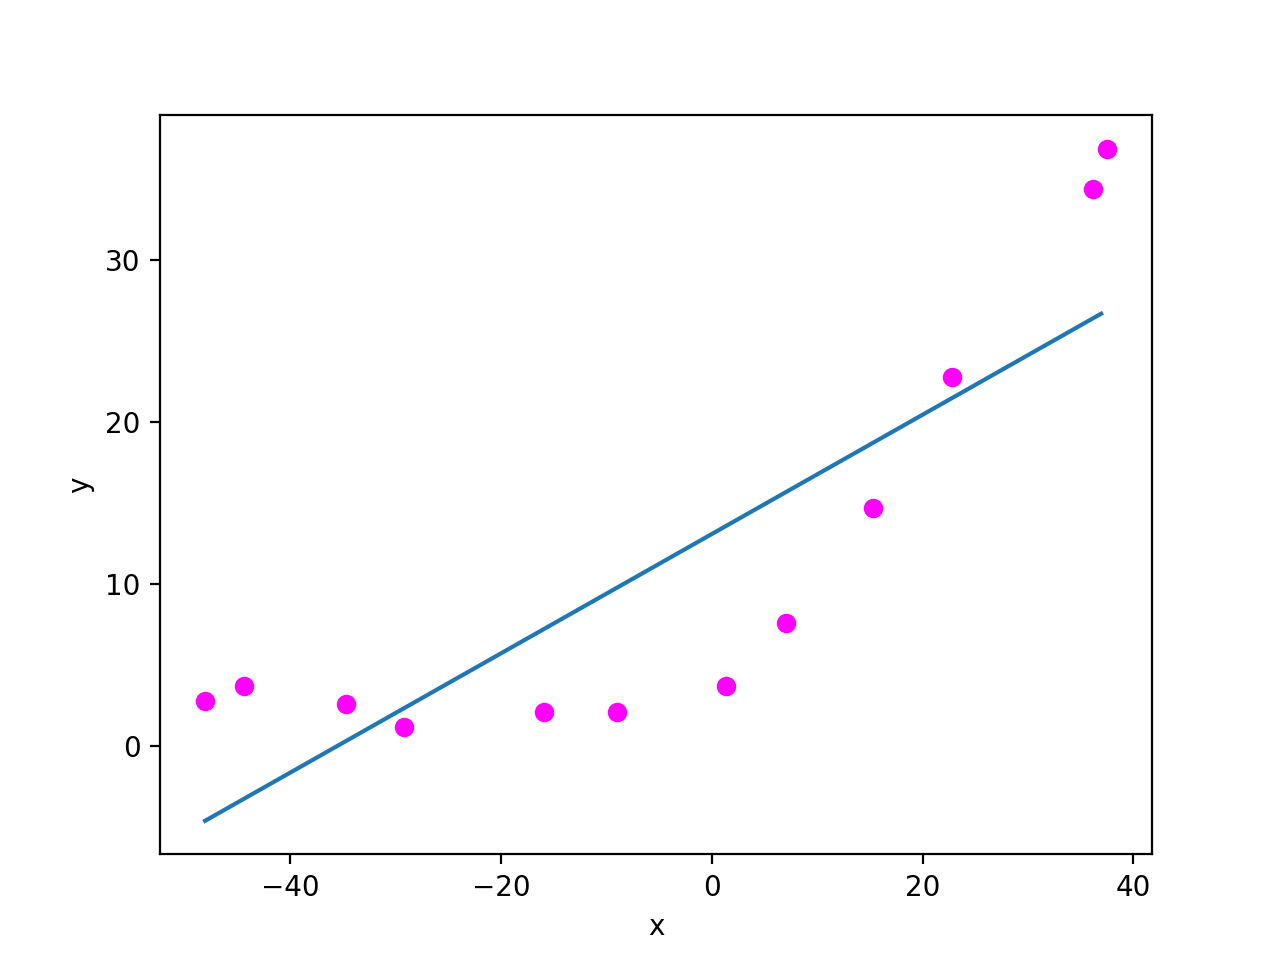
\includegraphics[width=0.5\linewidth]{figs/Chap_9_Figure_1.png}
\end{figure}


\paragraph{学习曲线的绘制}

绘制学习曲线时，依次增大训练集规模，每次重新训练参数，再分别计算当前训练子集的误差和验证集误差。需要注意，训练参数时可以使用正则化，但评估误差时应取 $\lambda=0$：

\begin{lstlisting}[language=Python]
Z_train = []
Z_valid = []
for i in range(1, 1+X.shape[0]):
	res = Train(X[:i, :], y[:i, :])
	Z_train.append(J(unseq(res.x), X[:i, :], y[:i, :], 0))
	Z_valid.append(J(unseq(res.x), Xval, yval, 0))

ax = plt.subplot(1, 1, 1)
ax.set_xlabel('size of training set')
ax.set_ylabel('Cost')
ax.set_title('learning curves')
ax.plot(range(1, 1+len(Z_train)), Z_train, color='darkviolet', label='Train')
ax.plot(range(1, 1+len(Z_valid)), Z_valid, color='tomato', label='Validation')
ax.legend()
plt.show()
\end{lstlisting}

作图如下：

\begin{figure}[H]
    \centering
    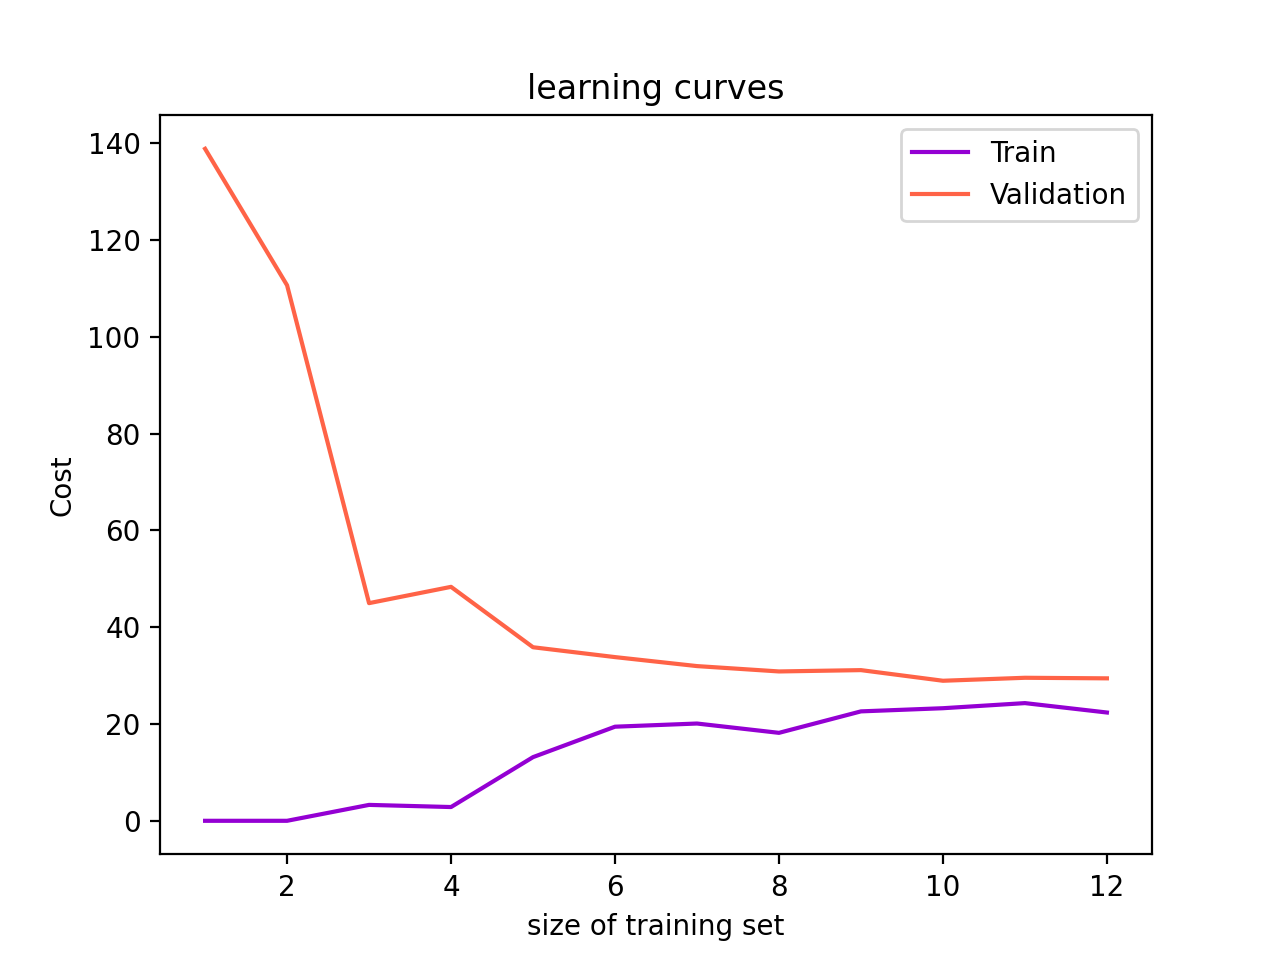
\includegraphics[width=0.5\linewidth]{figs/Chap_9_Figure_2.png}
\end{figure}

图中训练误差和验证误差都较大，并且随着样本数量增加逐渐接近。这是典型的高偏差学习曲线，说明当前线性模型发生了欠拟合。

\paragraph{多项式回归}

欠拟合的主要原因是当前使用了线性回归，而数据明显呈现非线性关系。为了提高模型的表达能力，下面引入高次特征，改用多项式回归。

加入高次特征后，特征取值范围会随着次数迅速增大，不同维度的尺度可能相差悬殊。为了保证优化过程稳定，需要对扩展后的特征进行标准化：

\begin{lstlisting}[language=Python]
data = loadmat('ex5data1.mat')
X, y, Xval, yval, Xtest, ytest = \
data['X'], data['y'], data['Xval'], data['yval'], data['Xtest'], data['ytest']

dim = 9
meanX, stdX = [], []
meany, stdy = 0, 0

def featurePrepare(X, y):
	"""
	feature extension & normalization
	"""
	global meanX, stdX, meany, stdy
	res = np.empty((X.shape[0], 0))
	for i in range(dim):
		tmpX = X ** i
		meanX.append(np.mean(tmpX, axis=0))
		stdX.append(np.std(tmpX, axis=0))
		if i:
			tmpX = (tmpX - meanX[i]) / stdX[i] if stdX[i] else tmpX - meamX[i]
		res = np.hstack((res, tmpX))
	meany = np.mean(y, axis=0)
	stdy = np.std(y, axis=0)
	y = (y - meany) / stdy if stdy else y - meany
	return res, y
\end{lstlisting}

首先使用最高次数为 $8$ 的多项式，并取正则化参数 $\lambda=0$. 此时模型具有较强表达能力，但完全没有正则化约束。拟合结果和学习曲线如下：

\begin{figure}[H]
    \centering
    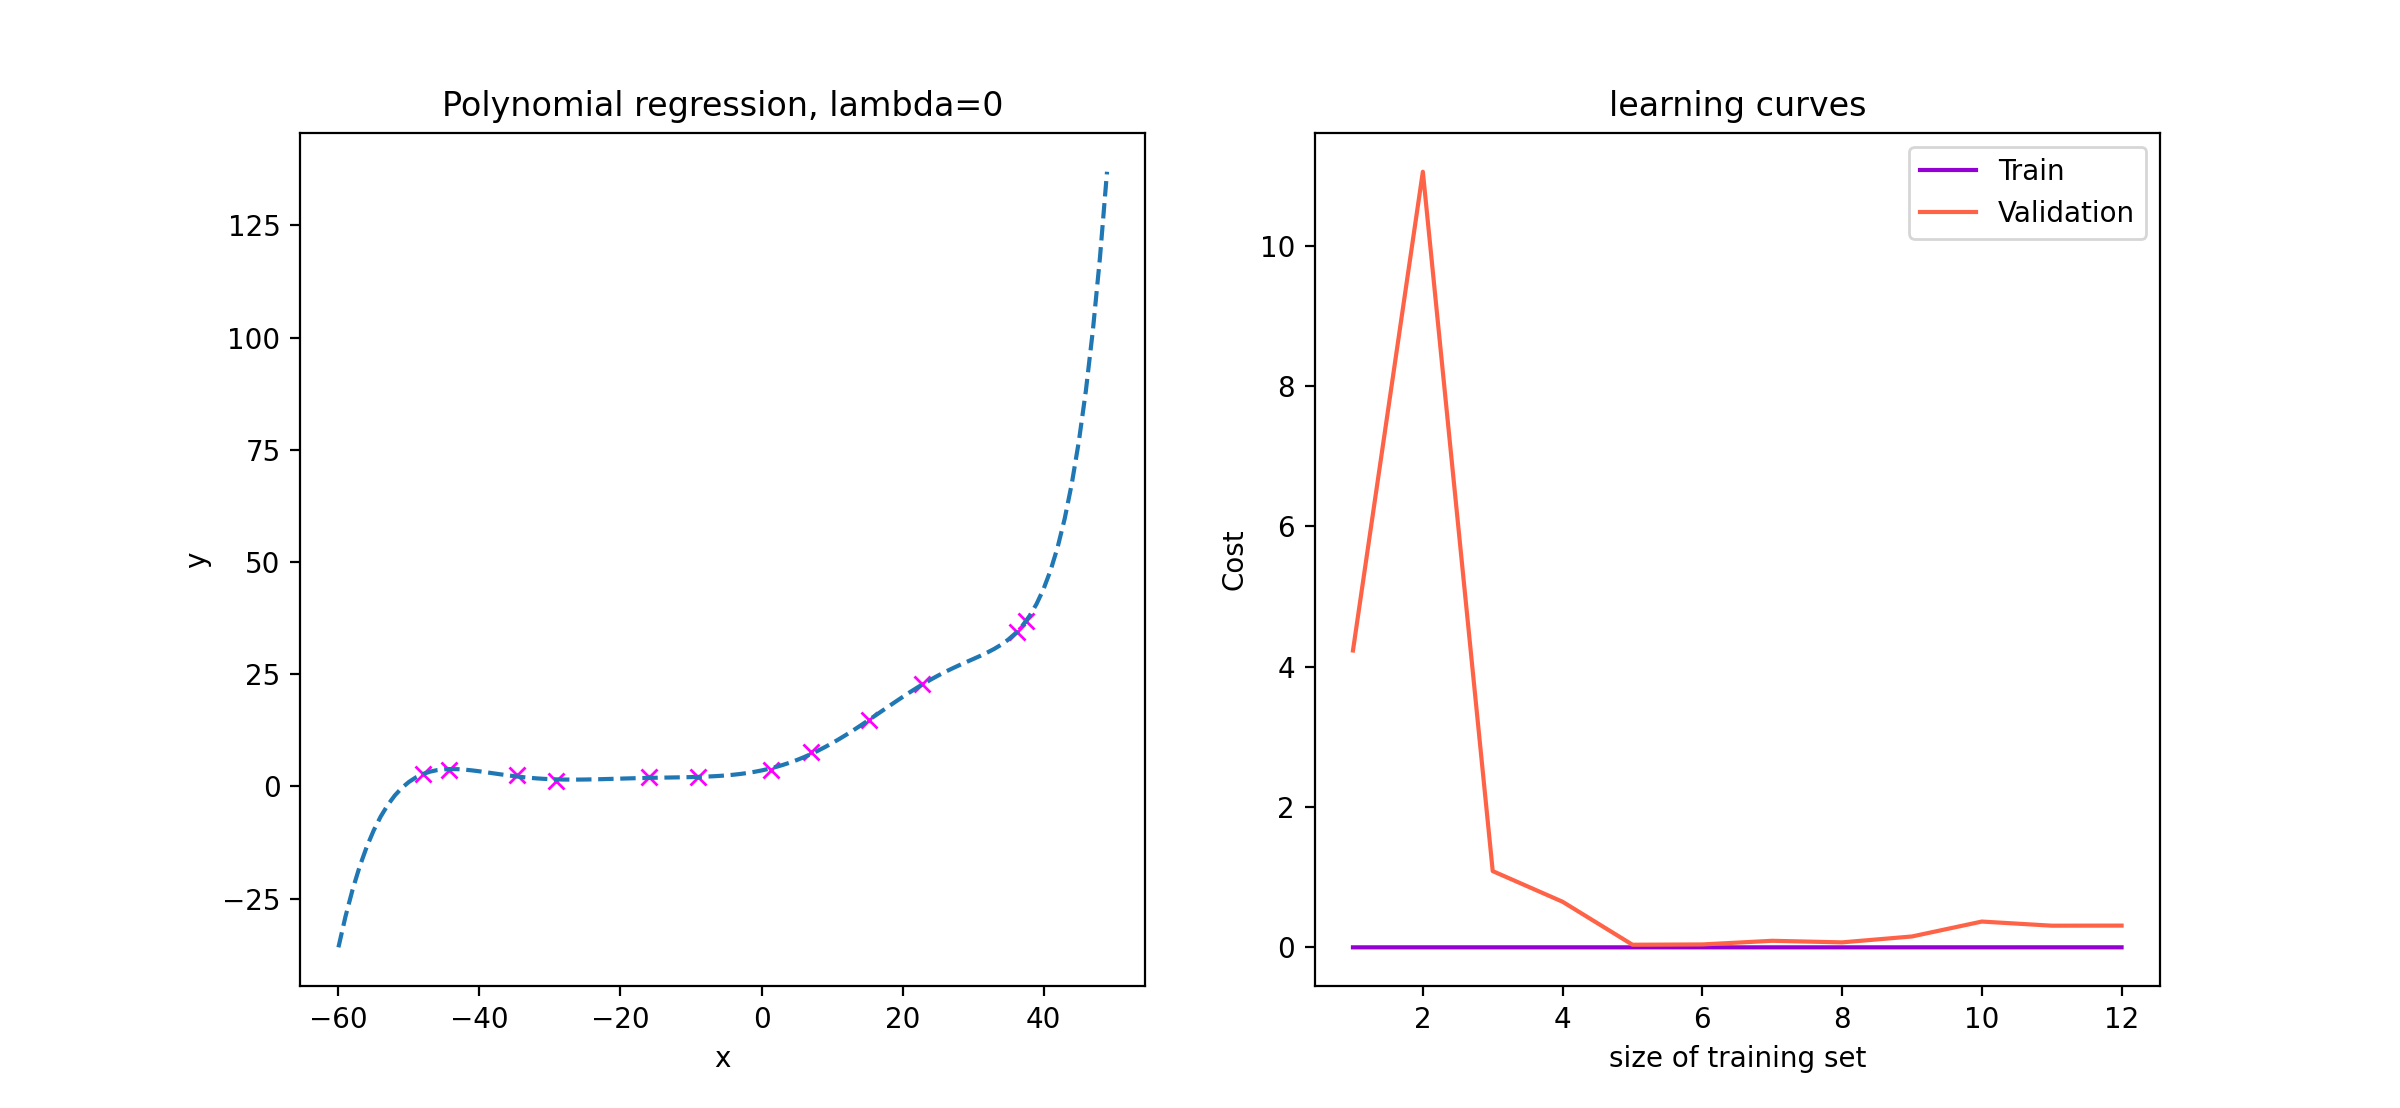
\includegraphics[width=0.8\linewidth]{figs/Chap_9_Figure_4.png}
\end{figure}
此时模型出现过拟合。

取 $\lambda=1$，得到拟合效果和学习曲线如下：
\begin{figure}[H]
    \centering
    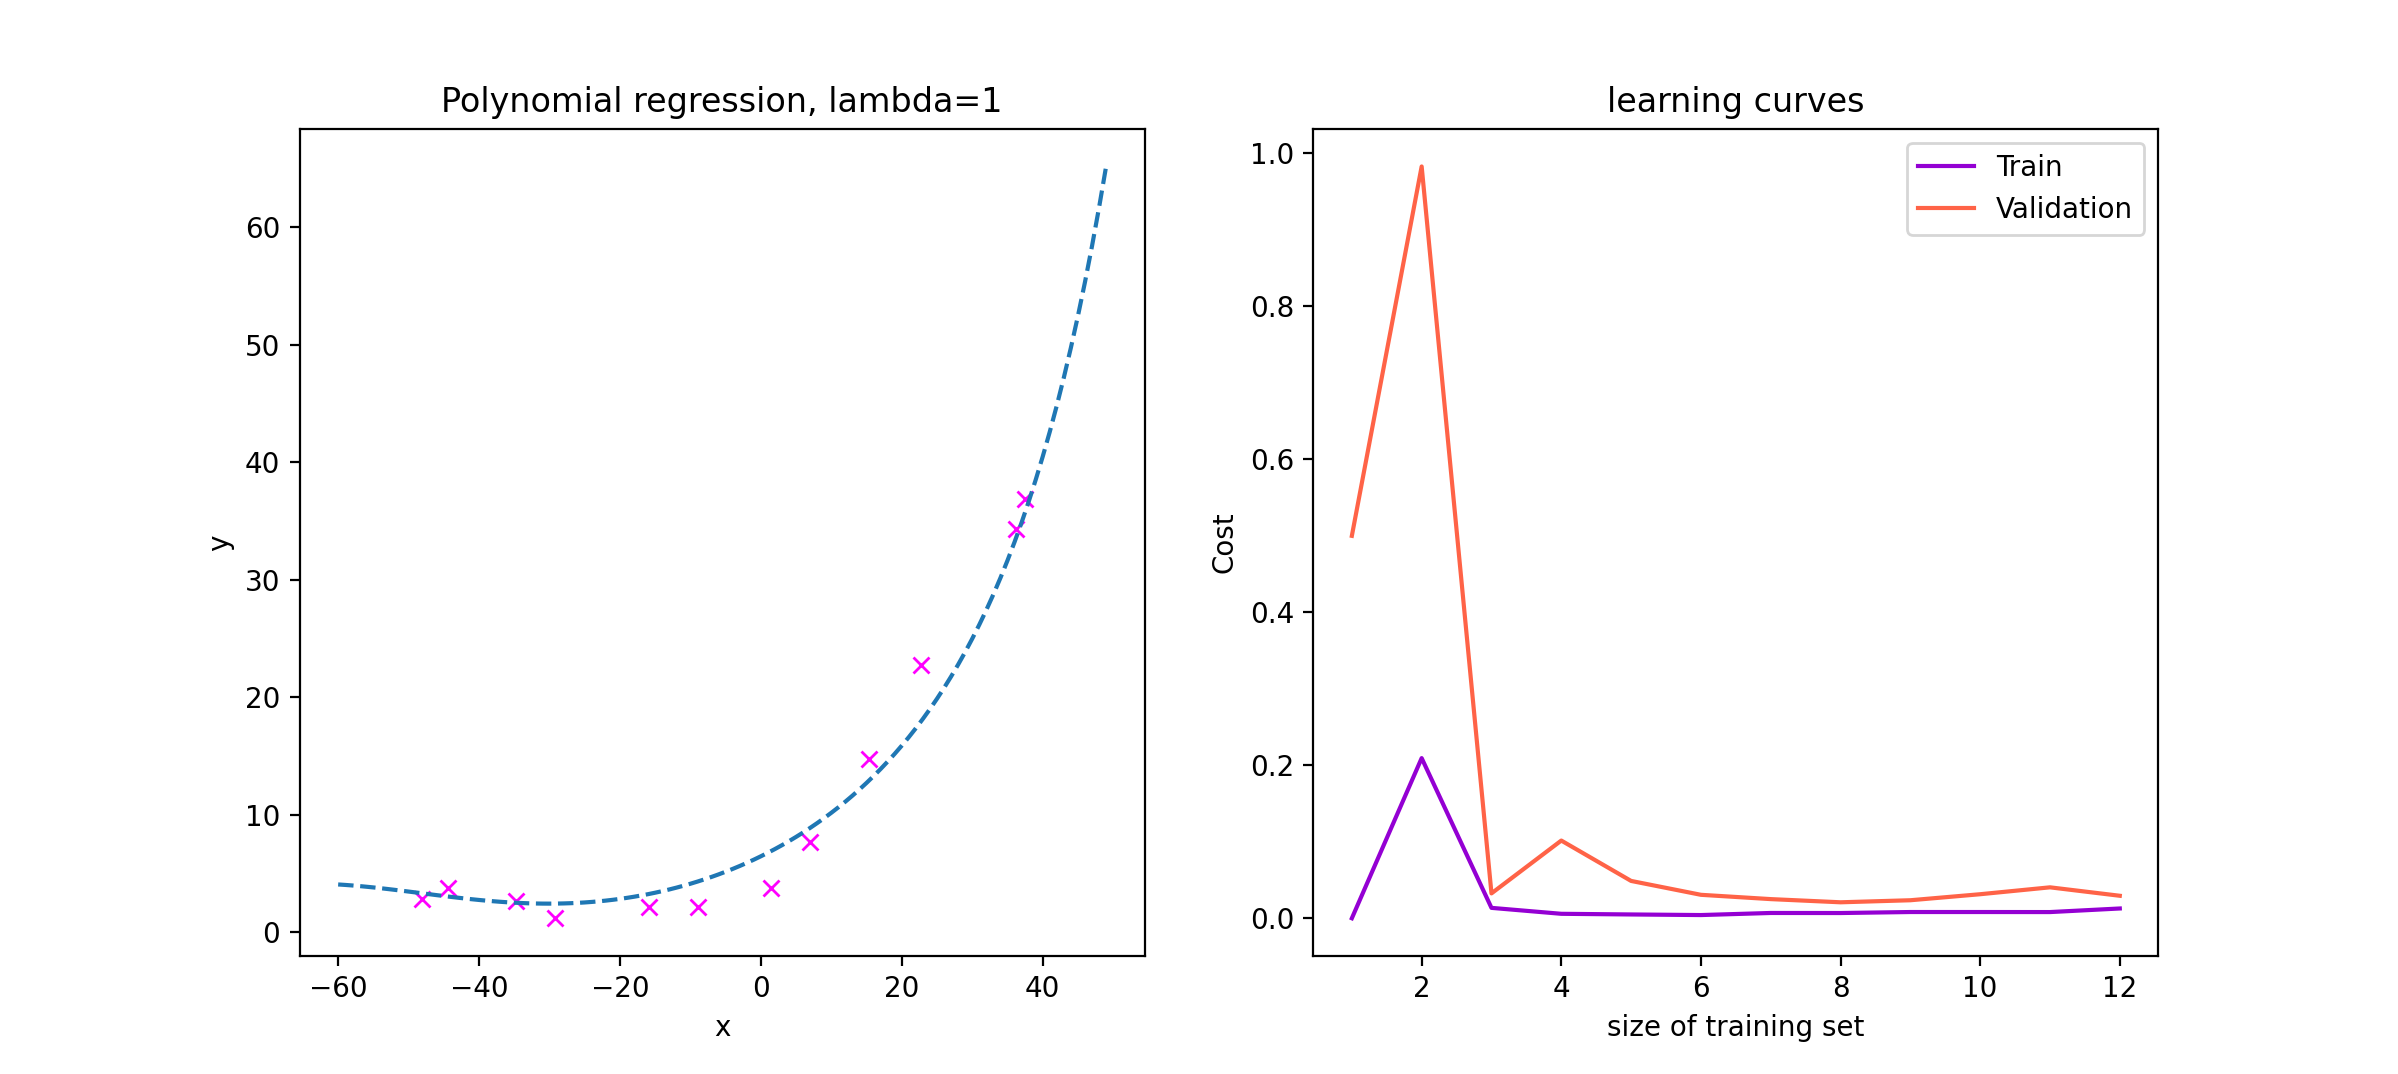
\includegraphics[width=0.8\linewidth]{figs/Chap_9_Figure_5.png}
\end{figure}
取 $\lambda=50$，得到拟合效果和学习曲线如下：
\begin{figure}[H]
    \centering
    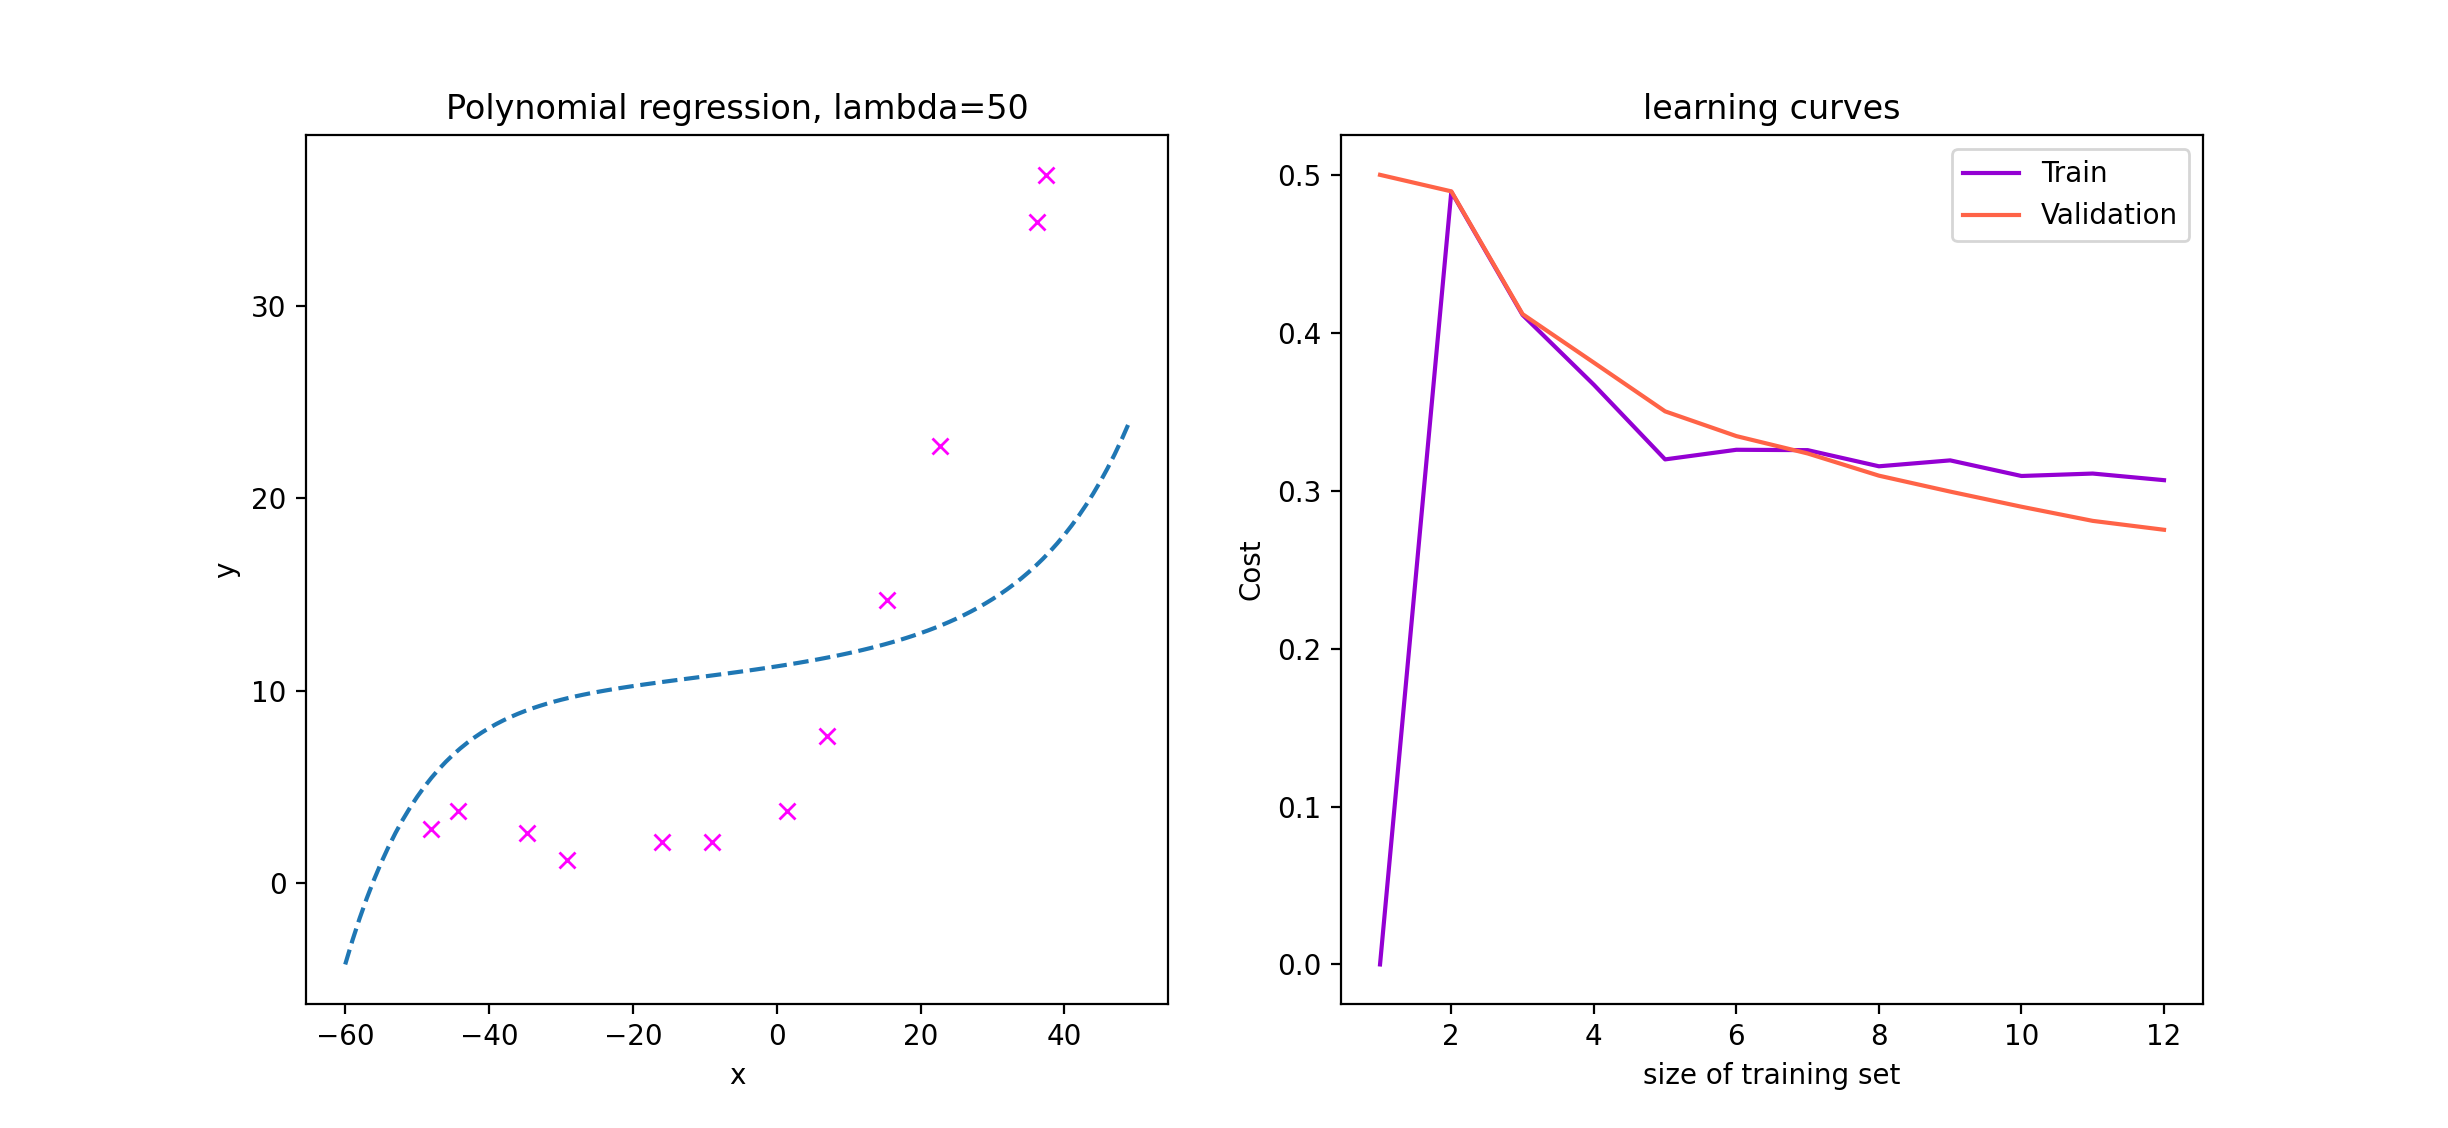
\includegraphics[width=0.8\linewidth]{figs/Chap_9_Figure_6.png}
\end{figure}
此时模型出现欠拟合。

为了系统选择正则化参数，接下来依次使用若干 $\lambda$ 训练模型，结果如下：

\begin{figure}[H]
    \centering
    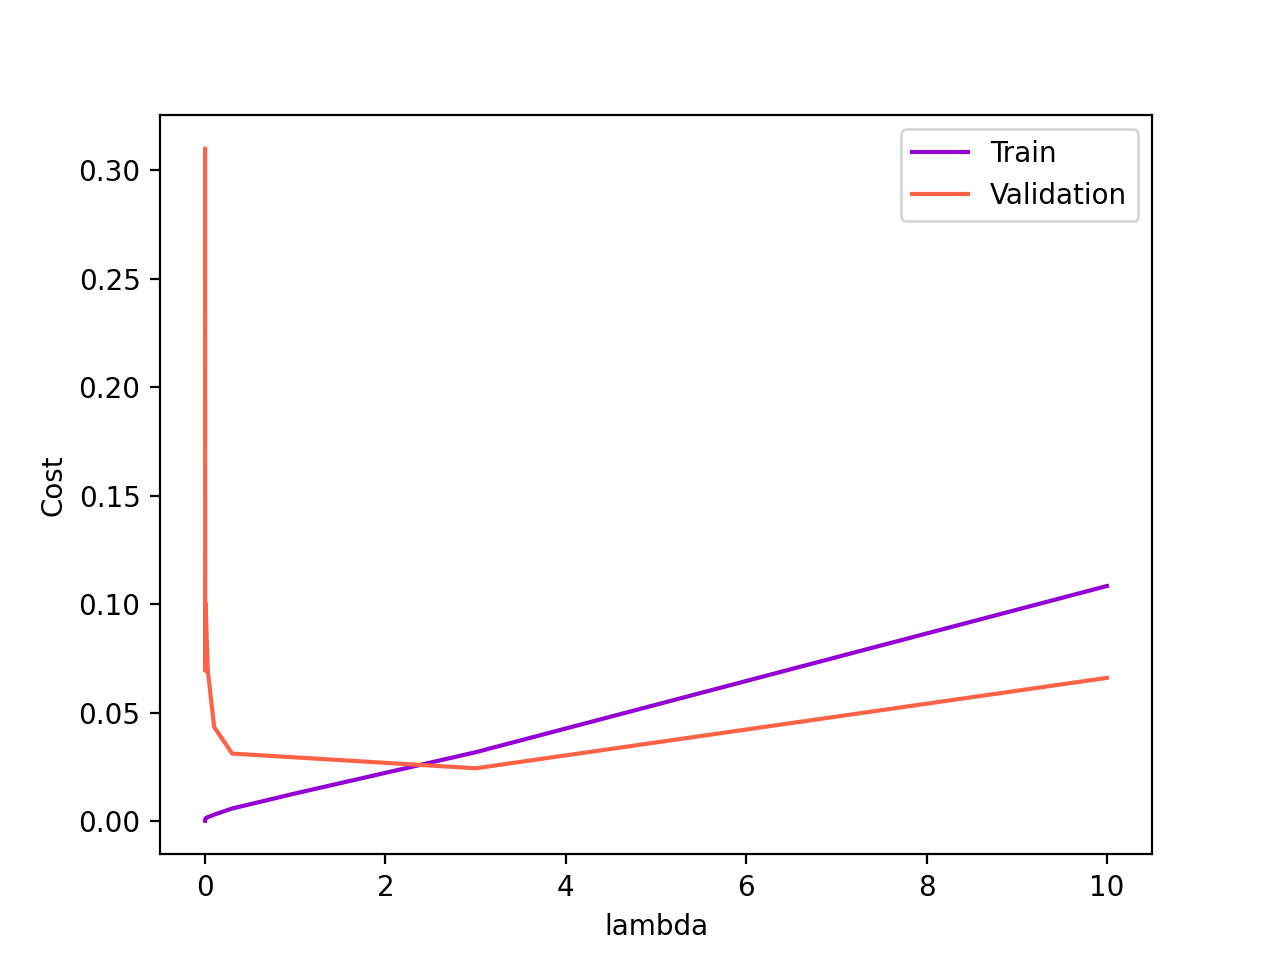
\includegraphics[width=0.5\linewidth]{figs/Chap_9_Figure_7.png}
\end{figure}

由图可见，较小的 $\lambda$ 容易产生高方差，较大的 $\lambda$ 又会带来高偏差；当 $\lambda=3$ 时验证误差最小，因此最终选取 $\lambda=3$. 
此时测试误差为 $J_\text{test}(\theta)=0.01393303991254464$. 
